\documentclass[technote,onecolumn,draftcls,12pt]{IEEEtran}

\usepackage{bm,bbm}
\usepackage{amsmath,amssymb}
\usepackage{graphicx,subfigure}
\usepackage{url}
\usepackage{units}
\usepackage{cite,balance}
\usepackage{comment}
\usepackage{multirow}
\usepackage{booktabs}
\usepackage{microtype}
\usepackage{siunitx}
\usepackage{color}
\usepackage{enumerate}
\usepackage{stackrel}

\usepackage[normalem]{ulem} %%%% para tachar texto

\newtheorem{definition}{Definition}
\newtheorem{proposition}{Proposition}
\newcommand{\at}[2][]{#1|_{#2}}

%%%%% EQUATIONS %%%%%%%%%%%%%%%%%%%%%%%%%%%%%%%%%%%

\numberwithin{equation}{section}

%%%%% THEOREMS %%%%%%%%%%%%%%%%%%%%%%%%%%%%%%%%%%%%%

\newtheorem{corollary}{Corollary}[section]
\newtheorem{lemma}{Lema}[section]
\newtheorem{theorem}{Theorem}[section]

%%%%% PROOFS %%%%%%%%%%%%%%%%%%%%%%%%%%%%%%%%%%%%%%%%

\newenvironment{dem}[1][Proof]{\begin{proof}[{\it #1}]}{\end{proof}}

%%%%% DEFINITIONS %%%%%%%%%%%%%%%%%%%%%%%%%%%%%%%%%%%

%\theoremstyle{definition}

%\newtheorem{definition}{Definici\'{o}n}[section]
\newtheorem{example}{Ejemplo}[section]
\newtheorem{remark}{Observaci\'{o}n}[section]
\newtheorem{exercise}{Ejercicio}[section]
%{\swapnumbers\newtheorem{exercisestar}[exercise]{(*)}}

%%%%% NUMEROS %%%%%%%%%%%%%%%%%%%%%%%%%%%%%%%%%%%%%%%

\newcommand{\e}{\mathrm{e}}
\newcommand{\ii}{\mathrm{i}}
\renewcommand{\r}{\mathbf{r}}
\renewcommand{\d}{\mathrm{d}}
\newcommand{\al}{&\,}

%%%%% CONJUNTOS NUMERICOS %%%%%%%%%%%%%%%%%%%%%%%%%%%

\newcommand{\C}{\ensuremath{\mathbbm{C}}}
\newcommand{\N}{\ensuremath{\mathbbm{N}}}
\newcommand{\Q}{\ensuremath{\mathbbm{Q}}}
\newcommand{\R}{\ensuremath{\mathbbm{R}}}
\newcommand{\T}{\ensuremath{\mathbbm{\zeta}}} 
\newcommand{\Z}{\ensuremath{\mathbbm{Z}}}

%%%%% FUNCIONES %%%%%%%%%%%%%%%%%%%%%%%%%%%%%%%%%%%%%

\renewcommand{\Re}[1]{\ensuremath{\mathrm{Re}\pa{ #1 }}}
\renewcommand{\Im}[1]{\ensuremath{\mathrm{Im}\pa{ #1 }}}
\renewcommand{\ker}[1]{\ensuremath{\mathrm{Ker}\pa{ #1 }}}
\newcommand{\ran}[1]{\ensuremath{\mathrm{Ran}\pa{ #1 }}}
\newcommand{\inc}{\ensuremath{\iota}}
\newcommand{\sig}[1]{\ensuremath{\mathrm{sgn}\pa{ #1 }}}
\newcommand{\sop}[1]{\ensuremath{\mathrm{sop}\pa{ #1 }}}
\newcommand{\tr}[1]{\ensuremath{\mathrm{tr}\pa{ #1 }}}
\newcommand*{\bigtimes}{\mathop{\raisebox{-.5ex}{\hbox{\huge{$\times$}}}}}

%%%%% LLAVES %%%%%%%%%%%%%%%%%%%%%%%%%%%%%%%%%%%%%%%%

\newcommand{\abs}[1]{\ensuremath{\left| #1 \right|}}
\newcommand{\norm}[1]{\ensuremath{\left\| #1 \right\|}}
\newcommand{\pa}[1]{\ensuremath{\left( #1 \right)}}
\newcommand{\pro}[2]{\ensuremath{\pa{ #1,#2 }}}
\newcommand{\set}[1]{\ensuremath{\left\{ #1 \right\}}}

%%%%% ESPACIOS VECTORIALES %%%%%%%%%%%%%%%%%%%%%%%%%%%%%

\newcommand{\Rn}[1][n]{\ensuremath{\R^{#1}}}
\newcommand{\Cn}[1][n]{\ensuremath{\C^{#1}}}

%%%%% ESPACIOS FUNCIONALES %%%%%%%%%%%%%%%%%%%%%%%%%%%%%

\newcommand{\sch}[1][n]{\ensuremath{\mathcal{S}\pa{\Rn[#1]}}}
\newcommand{\lp}[2]{\ensuremath{L^{#1}\pa{\Rn[#2]}}}
\newcommand{\lpw}[2]{\ensuremath{L^{#1,w}\pa{\Rn[#2]}}}
\newcommand{\sob}[2]{\ensuremath{H^{#1}\pa{\Rn[#2]}}}
\newcommand{\hil}{\ensuremath{\mathrm{H}}}


\begin{document}

\title{Consistency of the minimum triangular distance estimator based on asymmetric kernel density for the $\mathcal G_I^0$ model}
\author{ Julia~Cassetti, Diego Rial, and Alejandro~C.~Frery,~\IEEEmembership{Senior Member}

%\thanks{This work was supported by Secretar\'ia de Pol\'iticas Universitarias (SPU), CNPq, and Fapeal.}

\thanks{Julia Cassetti \texttt{julia.cassetti@gmail.com} is with the  Instituto de Desarrollo Humano, Universidad Nacional de General Sarmiento, Pcia. de Buenos Aires, Argentina.}

\thanks{Diego Rial \texttt{drial@dm.uba.ar} is with the Facultad de Ciencias Exactas y Naturales, Departamento de Matem\'{a}tica, Universidad de Buenos Aires, Argentina and IMAS, CONICET, Argentina.}

\thanks{Alejandro C.\ Frery \texttt{acfrery@laccan.ufal.br} is with the Laborat\'orio de Computa\c c\~ao Cient\'ifica e An\'alise Num\'erica, Universidade Federal de Alagoas, 
Av. Lourival Melo Mota, s/n, 57072-900 Macei\'o -- AL, Brazil.} 
}

\maketitle

\begin{abstract}
	The $\mathcal{G}^0$ family of distributions has been widely used in recent years to analyze and interpret data from sensors with coherent illumination, e.g., sonar, laser, ultrasound-B and synthetic aperture radar imagery.
	Special attention has been devoted to modeling data that come from images of Synthetic Aperture Radar (SAR) using a multiplicative model and the $\mathcal{G}^0$ distribution. 
	This law has positive support and is indexed by three parameters: texture, scale and number of looks.
	The estimation of the texture is of paramount importance, since it is able to characterize the kind of target under analysis.
	Many techniques have been proposed, among them maximum likelihood, analogy, robust methods and, more recently, minimum-distance estimators.
	In this paper we prove the consistency of the estimator based on the minimum Triangular Distance. 
	This estimator is defined as the argument that minimizes this stochastic distance between the theoretical distribution and a nonparametric estimation of the underlying density function based on an asymmetric kernel. 
	%Simulation study is presented comparing the performance of this estimator and the maximum likelihood one. We show that the former outperform the latter regarding bias and mean squared error, specially for small sample sizes.
%	This is considered an universal one because it has the ability to discriminate areas with different textures through one of its parameters. 
%	
%	
%Speckled images, such as SAR imagery, are well described by the $\mathcal G^0$ family of distributions because they possess the ability to characterize areas with different degrees of texture. 
%In the monopolarized case, this distribution depends on three parameters: the texture, the scale and the number of looks.
%The latter can be considered known because \textcolor{red}{\sout{it can be}} \textcolor{blue}{it is possible to} set up during the image generation process, or estimated for the whole image.
%The scale can be easily estimated as it depends on the mean value.
%The first one is related to the texture of the image, so its estimation deserves special attention.
%\textcolor{red}{\sout{This paper proposes and compares methods for the estimation of the texture parameter in intensity format.
%For the multilook case, the texture parameter is estimated by minimizing a stochastic distance between $\mathcal G^0$ density and an estimate of the underlying density function.}}
%\textcolor{red}{This paper proposes and compares methods for the estimation of the texture parameter in intensity format for the multilook case. The propose is estimate the texture parameter by minimizing a stochastic distance between $\mathcal G^0$ density and an estimate of the underlying density function using asymmetric kernels.}
%The Gamma and Lognormal asymmetric kernels are evaluated along with the cross-validation method to find the appropriate bandwidth.
%The properties of these estimators are assessed with analytic results and simulation studies. \textcolor{green}{VER!!}
%The new estimators outperform the maximum likelihood estimator regarding bias and mean squared error.
%We apply these estimators to actual images, with the purpose of identifying areas with different textures, using windows of several sizes to compare their performance. 
\end{abstract}

\begin{keywords}
Minimum distance estimator, stochastic distance, texture analysis, kernel estimation, synthetic aperture radar.
\end{keywords}

\IEEEpeerreviewmaketitle

\section{Introduction}
\label{intro}
\PARstart{S}{ynthetic} Aperture Radar (SAR) images are an important tool in
remote sensing. 
They are very useful for detection of deforested areas, crop characterization and oil spills in the sea, among other applications. 
%
They can be obtained regardless of weather conditions and sunlight, but this kind of images is contaminated by an interference pattern that makes difficult their interpretation. 
Such pattern, called \textit{speckle}, can be treated as noise and is inherent to the process of image capture. 
Images obtained from systems with coherent illumination such as laser, SAR, and ultrasound-B suffer from this type of noise.

Statistical modeling of SAR images has become an essential tool for analyzing and interpreting data with speckle. 
%%% ACF Si el párrafo anterior dirige la atención del lector al modelo multiplicativo, en este no se puede volver atrás. Organizar mejor, y no confundir la lectura entre amplitud e intensidad; sugiero trartar sólo intensidad.
A number of distributions has been proposed for modelling this kind of images. 
Log-Normal and Weibull were introduced to caractherize high resolution data~\cite{oliverquegan98}, 
\textit{K} and Weibull were considered in~\cite{Oliver1993}, 
in~\cite{Tison2004} the authors presented Fisher distribution to model several kinds of areas. 
Li et al.~\cite{Li2011} proposed a Generalized Gamma distribution for modeling SAR images 
which has the Weibull, \textit{K} and Fisher distributions, among others, as particular cases.

The multiplicative model has been successfully used to describe SAR data. 
It is based on the assumption that the return results from the product of two independent random variables: 
one corresponding to the backscatter (the unobserved truth) 
and the other to the speckle~\cite{oliverquegan98}. 
In recently years the $\mathcal G$ model~\cite{Frery97} has been widely utilized to depict the return of SAR images under this model, because it has the ability to discriminate textured and extremely textured areas better than other models~\cite{MejailJacoboFreryBustos:IJRS}. 
It is characterized by three parameters, the $\alpha$ parameter that models texture, the $\gamma$ parameter that informs about the brightness of the image, the number of looks $L$ is related to the signal-to-noise ratio. 
Due to this interpretability, quality parameter estimation is crucial, in particular for $\alpha$.

Sundry authors have studied the problem of parameter estimation for the $\mathcal G^0$ family. 
Freitas et al.~\cite{Freitas2005} used first and second for intensity data ($\mathcal G_I^0$) to estimate the texture and scale parameters. 
Vasconcellos et al.~\cite{VasconcellosFrerySilva:CompStat} proposed a second order correction for the bias in the estimation of the texture parameter for amplitud data ($\mathcal G_A^0$).  
Li et al~\cite{Li2011} obtained an expression for the estimators of the generalized Gamma distribution based on second-kind cumulants and a second-order approximation of the Polygamma  function. 
Cribari-Neto et al.~\cite{CribariFrerySilva:CSDA} implemented resampling techniques to improve the parameter estimation for the $\mathcal G_I^0$ model. 

Robustness is an important property. 
Bustos et al.~\cite{BustosFreryLucini:Mestimators:2001} and Allende et al.~\cite{AllendeFreryetal:JSCS:05} proposed M and AM estimators to improve the performance of maximum likelihood estimator under contamination. 
They showed that their proposals outperform the performance of maximum likelihood estimator, but they suffer from numerical problems specially with small samples. 

Nicolas and Anfinsen~\cite{nicolas2002} studied parameter estimation based on logmoments and logcumulants. 
These methods hinge on the relation between the moments of the distribution and the Mellin transform. 
The same idea was applied by Khan and Guida~\cite{khan2014} to estimate the parameters for the multivariate $\mathcal{G}$ model in polarimetric SAR data, and by Tison et al.~\cite{Tison2004} for estimation under the $\mathcal G_A^0$ model. 

Information Theory provides measure, called divergence, for comparing two density functions. 
They have been studied in the literature and have multiple applications in 
signal and image processing~\cite{SequentialCorrespondenceKernel}, 
medical image analysis diagnosis~\cite{5599869}, 
automatic region detection in SAR images~\cite{EdgeDetectionDistancesEntropiesJSTARS,SARSegmentationLevelSetGA0}, 
as a contrast measure to distinguish two image regions~\cite{Nascimento2009}, 
to obtain expressions for test statistics~\cite{ClassificationPolSARSegmentsMinimizationWishartDistances} among others.
Basu et al.~\cite{Basu2011} studied density-based distances with special attention to the Hellinger distance, as well as problems referred to hypothesis test based on divergences.

Minimum Distance Estimators (MDEs) are an alternative avenue with good properties for the problem of parameter estimation.
They come from the idea of finding a parameter estimator as the value that minimizes some  distance measure between the empirical and the theoretical distribution functions. 
Wolfowitz~\cite{wolfowitz1953,wolfowitz1957} studied this class of estimators and proved strongly consistency under general conditions. 
Boos studied~\cite{Boos1981} a weighted Cramer-von Mises distance between the empirical distribution function and the true model. 
The author showed that these estimators are consistent and asymptotically efficient under certain weight function. 
Hettmansperger et al.~\cite{HettmanSperger1994} studied unweighted minimum distance estimators in a location-scale model generated from the Cramer-von Mises distance. 
The author showed that these estimators are asymptotically normal, and have good efficiency properties as well as good robustness properties.
Beran ~\cite{beran1977} studied the problem of estimating the proportion of mixtures in a nonparametric mixture model. 
The author addressed this problem using a minimum Hellinger distance estimator between a parametric mixture model and a nonparametric density estimator, and proved important properties such us strong consistency, asymptotic normality and asymptotic efficiency.  
Parr and Schucany~\cite{parr1982} proved that, under certain conditions, the minimum distance estimator between empirical distribution function and the theoretical distribution function are  consistent.

Beran~\cite{beran1977} studied the properties of MDEs estimator, but the minimization is between the true density model and an appropriate nonparametric density estimator of the underlying density function. 
Asymptotic and robustness properties were examined using the Hellinger distance. 
Cao et al.~\cite{cao1995minimum} proposed minimizing a distance between the theoretical density function and an estimator of the underlying density function using the classical symmetric kernel estimator to obtain minimum distance estimators. 
They proved, following~\cite{parr1982}, the strong consistency of these estimators under certain considerations, and also studied their asymptotic normality for the case of the $L_2$ metric.

%In~\cite{beran1977} the author studies asymptotic and robustness properties of the minimum Hellinger distance estimator. 
%In~\cite{Boos1981} a Cramer-von Mises distance with a weighted function is used to obtain asymptotically efficient estimators that arise from minimize this distance.


%\textcolor{blue}{These stochastic distance are used in~\cite{Nascimento2009} as a contrast measure to distinguish two image regions. Analytic expressions for test statistics based on stochastic distances were obtained in~\cite{ClassificationPolSARSegmentsMinimizationWishartDistances}, where the authors also proposed new classifier for Polarimetric SAR images using these distances. Many information on theoretic divergences measures are described in~\cite{Liese2006}.
% }
Gambini et al.~\cite{gambini2015} proposed an estimator of the texture parameter of the $\mathcal{G}_I^0$ distribution by combining MDEs with stochastic distances. 
They proposed minimizing the triangular stochastic distance between the theoretical density function and an estimation of the underlying density function using asymmetric kernels; in this case, the Inverse Gaussian kernel. 
The authors compared its performance with logcumulant and maximum likelihood estimators, and obtained good results in terms of mean squared error, bias, consistency and robustness by means of a Monte Carlo study. 
No theoretical results were shown.

In this work we prove the consistency of the estimator presented in~\cite{gambini2015} and we generalized this result to other asymmetric kernels.
A proof of this property is missing in the literature, and gives more confidence to the use of this class of estimators.

The rest of the paper unfolds as follows: 
Section~\ref{sec_SAR} recalls the main features of the $\mathcal{G}_I^0$ model.
Section~\ref{DTsection} presents the triangular distance and some theoretical results. 
Section~\ref{AK} defines and shows main results of asymmetric kernel estimator.
In Section~\ref{MDE} we present the consistency results of the minimum distance estimator. 
Finally, we draw our conclusions in Section~\ref{conclusions}.

\section{The $\mathcal{G}_I^0$ Model}
\label{sec_SAR}
Images generated from devices that employ coherent illumination are contaminated with speckle. 
It is known that this kind of interference pattern can be modeled as noise, but neither Gaussian nor additive. 

SAR images can be modeled as the product of two independent random variables, one corresponding to the backscatter $X$ and other to the speckle noise $Y$. In this manner $Z=X Y  $ represents the return $Z$ in each pixel under the multiplicative model.
The speckle noise in intensity format $Y$ is modeled as a $\Gamma $ random variable with unitary mean and shape parameter $L\geq1$, which is proportional to the signal-to-noise ratio and is called ``number of looks''. 

%The multiplicative model with the $\mathcal{G}_I^{0}$ law is a good combination to successfully describe areas with varying degrees of texture~\cite{Frery97,MejailJacoboFreryBustos:IJRS}. 
The backscatter $X$ can be modeled by a reciprocal of $\Gamma(\alpha,\gamma) $ law~\cite{Frery97,MejailJacoboFreryBustos:IJRS}. 
The $\alpha$ parameter is related to the texture of the image and is negative. 
The $\gamma$ parameter gives information of the brigthness of the image and is a positive value. This gives rise to the $\mathcal{G}_I^{0}$ distribution for the return $Z$.

The density function for intensity data, $\mathcal{G}_I^{0}$ is given by
\begin{equation}
f_{\alpha,\gamma,L}( z) =\frac{L^{L}\Gamma ( L-\alpha
	) }{\gamma ^{\alpha }\Gamma ( -\alpha ) \Gamma (
	L) }\cdot  
\frac{z^{L-1}}{( \gamma +zL) ^{L-\alpha }},%
\label{ec_dens_gI0}
\end{equation}
where $-\alpha,\gamma ,z>0$ and $L\geq 1$. 
The $r$-order moments are
\begin{equation}
\text{E}(Z^r) =\Big(\frac{\gamma}{L}\Big)^r\frac{\Gamma ( -\alpha-r )}{ \Gamma (-\alpha) }
\frac{\Gamma (L+r )}{\Gamma (L)},
\label{moments_gI0}
\end{equation}
provided $\alpha<-r$, and infinite otherwise.

It is important to obtain accurate and robust estimates of $\alpha$ because  it is related to the roughness or texture of the target. 
Values close to zero ($\alpha \in (0,-3)$) suggest extreme texture, as in urban areas. 
As the value decreases, the texture is also reduced going, usually, from $\alpha \in (-6,-3]$ in forest zones up to $\alpha\in(-\infty,-6)$ in textureless targets, e.g. pasture or crops.

The parameter $\gamma$ is proportional to the brightness, and is a scale parameter.
With the purpose of reducing our analysis to a single parameter, we based the forthcoming analysis on the condition $E(Z)=1$ which links the texture and the brightness parameter as $\gamma^* =-\alpha-1$.

\subsection{Some theoretical properties of the $\mathcal{G}_I^{0}$ model}
Consider $\Omega = \pa{-\infty,0}\times\pa{0,\infty}\times\pa{1,\infty}$
with the usual distance in $\Rn[3]$, for each $\pa{\alpha,\gamma,L}$ then:
%\begin{align*}
%f_{\alpha,\gamma,L}\pa{z} = \frac{\gamma^{-\alpha} L^{L} \Gamma\pa{L-\alpha}}{\Gamma\pa{-\alpha}\Gamma\pa{L}}
%\frac{z^{L-1}}{\pa{\gamma +L z}^{L-\alpha}},\quad z>0,
%\end{align*}

\begin{proposition}\label{pr: continuidad}
	Let $\mathcal{F}$ be the metric space given by the set of one-dimensional probability density functions with the metric $\norm{\cdot}$ of $L^{1}\pa{\R}$.
	The map from $\Omega$ in $\mathcal{F}$ given by 
	$\pa{\alpha,\gamma,L}\mapsto f_{\alpha,\gamma,L}$ is continuous, where $f_{\alpha,\gamma,L}$ is defined in~\ref{ec_dens_gI0}.
\end{proposition}

\begin{dem}
	Writing $f_{\alpha,\gamma,L}$ as
	\begin{align*}
	f_{\alpha,\gamma,L}\pa{z}= \frac{\Gamma\pa{L-\alpha}}{\Gamma\pa{-\alpha}\Gamma\pa{L}}
	\frac{L}{\gamma}\pa{\frac{Lz}{\gamma+Lz}}^{L-1}
	\pa{1+\frac{Lz}{\gamma}}^{-1+\alpha},
	\end{align*}
	and considering that $\pa{\frac{Lz}{\gamma+Lz}}^{L-1}<1$, it can be obtained that
	$f_{\alpha,\gamma,L}\pa{z} \le c_{\alpha,\gamma,L} \pa{1+\frac{Lz}{\gamma}}^{-1+\alpha}$, where
	\begin{align*}
	c_{\alpha,\gamma,L} = \frac{\Gamma\pa{L-\alpha}}{\Gamma\pa{-\alpha}\Gamma\pa{L}}
	\frac{L}{\gamma}.
	\end{align*}
	
	Let $\pa{\alpha,\gamma,L}\in\Omega$, $0<\varepsilon<1-1/L$, 
	the compact neighborhood is defined as
	\begin{align*}
	Q=\set{\pa{\alpha',\gamma',L'}\in\Omega:
		1-\varepsilon\le \textstyle{\frac{\alpha'}{\alpha},\frac{\gamma'}{\gamma},\frac{L'}{L}} \le 1+\varepsilon}.
	\end{align*}
	For $\pa{\alpha',\gamma',L'}\in Q$ it is verified that %$C = \max\limits_{\pa{\alpha',\gamma',L'}\in Q}c_{\alpha,\gamma,L}$, vale 
	$$
	f_{\alpha',\gamma',L'}\pa{z} 
	\le \max\limits_{{\alpha',\gamma',L'}\in Q}c_{\alpha',\gamma',L'}
	\left({1+\frac{\pa{1-\varepsilon}Lz}{\pa{1+\varepsilon}\gamma}}\right)^{-1+\pa{1-\varepsilon}\alpha} 
	= g\pa{z}.
	$$
	If $\pa{\alpha_{n},\gamma_{n},L_{n}}$ is a sequence in $\Omega$ such that $\pa{\alpha_{n},\gamma_{n},L_{n}}\stackrel[n\to\infty]{}{\longrightarrow}\pa{\alpha,\gamma,L}$, then for each $z>0$
	$f_{\alpha_{n},\gamma_{n},L_{n}}\pa{z}\stackrel[n\to\infty]{}{\longrightarrow} f_{\alpha,\gamma,L}\pa{z}$.
	As $g$ is an integrable function, by the dominated convergence theorem, it is verified that
	$\norm{f_{\alpha_{n},\gamma_{n},L_{n}} - f_{\alpha,\gamma,L}}\to 0$.
\end{dem}

It is assumed that  $L$ is known and $\alpha<-1$, which implies that the first moment exists and, 
%it is
%\begin{align*}
%m_{1} = \int_{0}^{\infty}z\,f_{\alpha,\gamma,L}\pa{z}dz = -\frac{\gamma}{\alpha+1}.
%\end{align*}
taking $\gamma = -\pa{\alpha+1}$, it is obtained $E(Z) = 1$.
So, we consider the reduced model $\set{f_{\alpha}:\alpha\in I}$,
where $I = \pa{-\infty,-1}\label{I}$ and, in the following, we will denote $f_{\alpha}$ instead of $f_{\alpha,-\pa{\alpha+1},L}$.
Notice that, with the relationship between $\alpha$ and $\gamma$, $f_{\alpha}$ can be written as
\begin{align}
f_{\gamma}(z)=\frac{\Gamma\pa{L+\gamma+1}}{\Gamma\pa{\gamma+1}\Gamma\pa{L}}
\pa{\frac{L}{\gamma}}^L \frac{z^{L-1}}{\pa{1+\frac{Lz}{\gamma}}^{L+\gamma+1}}.
\label{fgamma}
\end{align}

%\begin{align}
%f_{\gamma}(z)=\frac{\Gamma\pa{L+\gamma+1}}{\Gamma\pa{\gamma+1}\Gamma\pa{L}}
%\frac{L}{\gamma}\pa{\frac{Lz}{\gamma+Lz}}^{L-1}
%\pa{1+\frac{Lz}{\gamma}}^{-2-\gamma}
%\label{fgamma}
%\end{align}

The next two results show the uniform comvergence of $f_\alpha$ when $\alpha \to -\infty$ and $\alpha \to -1$.

\begin{proposition}
	For all compact interval $[z_{1},z_{2}]\subset\pa{0,\infty}$, $f_{\alpha}$ converges uniformly to $\Gamma_{(L,1/L)}$ in $[z_{1},z_{2}]$ if $\alpha\to -\infty$,
	where $\Gamma_{(L,1/L)}$ is the density function of the $\Gamma$ model with parameters $\pa{L,1/L}$.
	\label{pr: convergenciauniforme1}
\end{proposition}

\begin{dem}
	Notice that, studying the $\lim\limits_{\alpha\to-\infty} f_{\alpha}$ is equivalent to finding
	$\lim\limits_{\gamma\to+\infty} f_{\gamma}$.
From Stirling's formula~\cite{abramowitz1964}:
\begin{align*}
% \lim_{\gamma\to+\infty} a\pa{L,\gamma} = 
% \al \lim_{\gamma\to+\infty}\frac{\Gamma\pa{L+\gamma+1}\e^{L+\gamma}}{\sqrt{2\pi}\pa{L+\gamma}^{L+\gamma+1/2}} = 1,\\
\lim_{\gamma\to+\infty} a\pa{\gamma} = 
\al \lim_{\gamma\to+\infty}\frac{\Gamma\pa{\gamma+1}\e^{\gamma}}{\sqrt{2\pi}\gamma^{\gamma+1/2}} = 1,
\end{align*}
so
\begin{align*}
\lim_{\gamma\to+\infty} \frac{a\pa{L+\gamma}}{a\pa{\gamma}} = 
\lim_{\gamma\to+\infty}\frac{\Gamma({L+\gamma+1})}{\Gamma\pa{\gamma+1}}
 \; \e^{L}\gamma^{-L}\left({1+\frac{L}{\gamma}}\right)^{-L-\gamma-1/2}
= 1.
\end{align*}

On the other hand, it is verified that
\begin{align*}
\lim_{\gamma\to+\infty} b\pa{L,\gamma,z} =
\al \lim_{\gamma\to+\infty}L\gamma^{L-1}\pa{\frac{Lz}{\gamma+Lz}}^{L-1} \\
= \al \lim_{\gamma\to+\infty} \frac{L^{L} z^{L-1}}{\pa{1+\frac{Lz}{\gamma}}^{L-1}} = L^{L} z^{L-1},\\
\lim_{\gamma\to+\infty} c\pa{L,\gamma,z} = \al \lim_{\gamma\to+\infty}\pa{1+\frac{Lz}{\gamma}}^{-2-\gamma} = \e^{-Lz},
\end{align*}
	
where the convergence is uniform in $[z_{1},z_{2}]$.
	
Being that
\begin{align*}
f_{\gamma}\pa{z} = \frac{a\pa{L+\gamma}}{a\pa{\gamma}\Gamma\pa{L}}\e^{-L}\pa{1+\frac{L}{\gamma}}^{L+\gamma+\frac 1 2}
b\pa{L,\gamma,z}c\pa{L,\gamma,z},
\end{align*}
%\begin{align*}
%	f_{\gamma}\pa{z} = \frac{a\pa{L+\gamma}}{a\pa{\gamma}\Gamma\pa{L}}\e^{L}\pa{1+\frac{L}{\gamma}}^{-L-\gamma-\frac 1 2}
%	b\pa{L,\gamma,z}c\pa{L,\gamma,z}
%	\end{align*}
	then $\lim\limits_{\gamma\to-\infty} f_{\gamma}\pa{z} = L^{L}/\Gamma\pa{L}\,\e^{-Lz}z^{L-1}$
	is obtained uniformly in $[z_{1},z_{2}]$.
\end{dem}

Fig.~\ref{ConvInfinito} illustrates the uniform convergence of $f_{\alpha}$ to $\Gamma(3,1/3)$, when $\alpha \to -\infty$ and $L=3$. 
The gray area is a band of width $\epsilon=0.1$ around the $\Gamma(3,1/3)$ density function (solid line). 
The dotted and twodash lines represent $f_{\alpha}$ density function for $\alpha=-20$ and $\alpha=-8$ respectively. 
It can be seen that, as the value of $\alpha$ becomes smaller, the $f_{\alpha}$ density function falls inside the gray area. 
Even more, for this value of $\epsilon$, $f_{-20}$ already falls within that band.

\begin{figure}[hbt]
	\centering    
	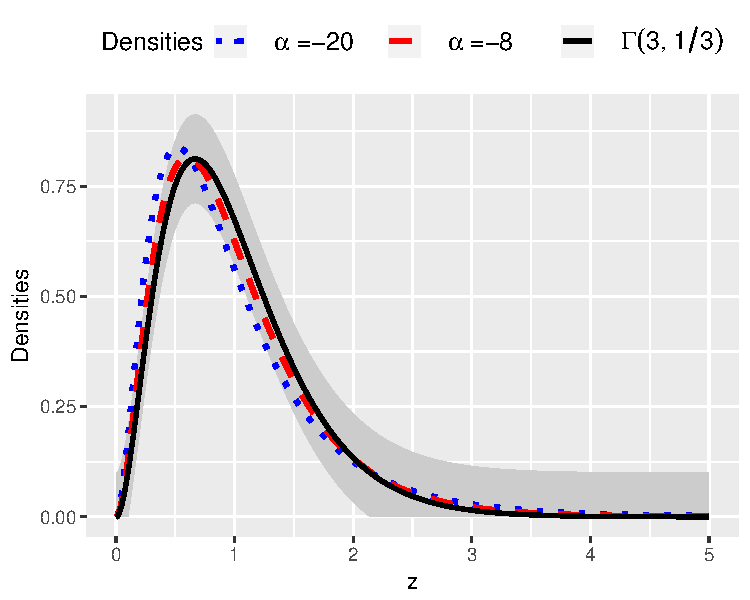
\includegraphics[width=\linewidth]{../../../Figures/DTTeorico/ConvUniformeMenosInfinito2.pdf}
	\caption{\label{ConvInfinito}Uniform convergence of $f_{\alpha}$, to $\Gamma(3,1/3)$, when $\alpha \to -\infty$, $L=3$ and $\epsilon=0.1$.}
\end{figure} 

\begin{proposition}
	For all compact interval $[z_{1},z_{2}]\subset\pa{0,\infty}$, $f_{\alpha}$ converges uniformly to $0$ in $[z_{1},z_{2}]$ when $\alpha\to -1^{-}$.
	\label{pr: convergenciauniforme2}
\end{proposition}

\begin{dem} 
	Due to the relationship between $\alpha$ and $\gamma$, study the $\lim\limits_{\alpha\to-1} f_{\alpha}$ is equivalent to finding
	$\lim\limits_{\gamma\to0} f_{\gamma}.$
	From~\eqref{fgamma}:
	\begin{align*}
	 f_{\gamma}\pa{z} = &\frac{\Gamma\pa{L+\gamma+1}}{\Gamma\pa{\gamma+1}\Gamma\pa{L}}
	L^{L} \frac{z^{L-1}}{(\gamma+LZ)^{L+\gamma+1}} \gamma^{\gamma +1}  \\
	\leq& \frac{\Gamma\pa{L+\gamma+1}}{\Gamma\pa{\gamma+1}\Gamma\pa{L}}
	L^{L} \frac{z_2^{L-1}}{(\gamma+Lz_1)^{L+\gamma+1}} \gamma^{\gamma +1} 
	\end{align*}
	Given that $\Gamma$ is a continuous function, for $z \in [z_{1},z_{2}]$, $\lim\limits_{\gamma\to0} f_{\gamma}=0$ uniformly in $z$. So the result is obtained.
\end{dem}

\begin{figure}[hbt]
	\centering    
	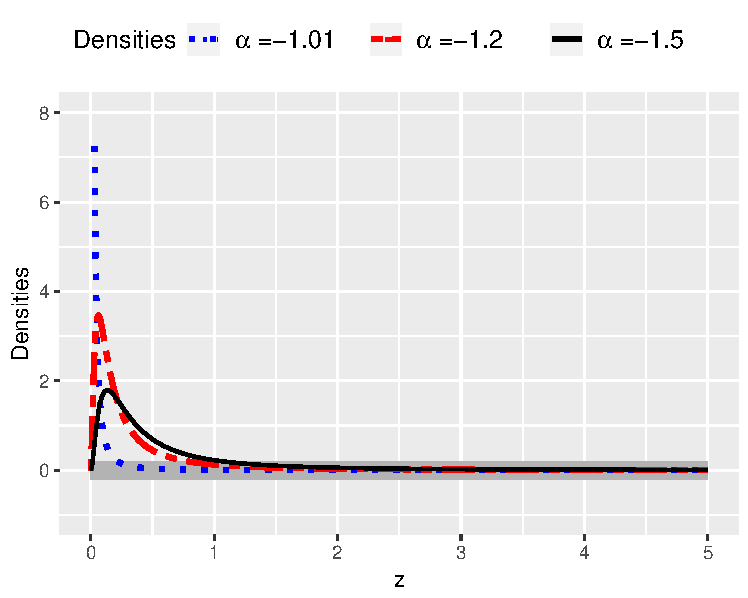
\includegraphics[width=\linewidth]{../../../Figures/DTTeorico/ConvUnifEnCero.pdf}
	\caption{\label{ConvEnCero}Uniform convergence of $f_{\alpha}$, to $0$, when $\alpha \to -1$, $L=3$ and $\epsilon=0.1$.}
\end{figure}

Fig.~\ref{ConvEnCero} illustrates the uniform convergence of $f_{\alpha}$ when $\alpha \to -1$. 
In this case, the gray band is of width $\epsilon=0.2$, around the $z$ axes. 
Three different densities where plotted: dotted, twodashed and solid which represent $f_{\alpha}$ density functions for $\alpha=-1.01, \ -1.2$ and $-1.5$ respectively. 
It can be seen that as the value of $\alpha$ gets closer to $-1$, $f_{\alpha}$ flattens to zero, except for $z=0$. 
For  $\epsilon=0.2$ and any interval $[z_1,z_2]$ is considered, $f_{\alpha}$ falls inside the band of width $\epsilon=0.2$ for $\alpha$ small enough. 
For example, for the interval $[1.5,2]$ and for this value of $\epsilon$, $f_{\alpha}$ gets inside the grey band since $\alpha=-1.5$. 
If the interval is $[0.5,1]$ this happens since $\alpha=-1.01$.
%%%%%%%%%%%%%%%%%%%%%%%%%%%%%%%%%%%%%%%%%%%%%%%%%%%%%%%%%%%%%%%%%%%%%%%%%%%%%%%%%%%%%%%%%%%%%%%%%%%%%%%%%%%%%%%%%%%%%%%%%%%%%%%%%%%%%%%%%%%%%%%%%%%%%%%%%%%%%%%%%%
\section{Triangular Distance}
\label{DTsection}

Discrepancy measures have been deeply by a number of authors. 
Sahler~\cite{Sahler1970} defined a discrepancy measure between two probability measures to any non-negative function between them. 
Csisz\'ar~\cite{Csiszar1967} defined $f$-divergences and he introduced this definition as a generalization of the Kullback-Leibler divergence. 
Lin~\cite{Lin1991} studied divergence measures based on the Shannon entropy.  
Salicru et al.~\cite{Salicru1994} established a generalization of the $f$-divergences and defined the $(h,\phi)$-divergence between two density functions. 
If the divergence is also a symmetric function, it is called a stochastic distance or simply a distance.

Nascimento et al.~\cite{Nascimento2009} examined different stochastic distances symmetrizing $(h,\phi)$-divergences. 
In order to identify different areas in terms of their textured in SAR imagery, they assessed eight statistical tests based on stochastic distances under the $\mathcal{G}_I^0$ model. 
They obtained that the test based on the triangular contrast measure was the one that presented the best performance for heterogeneity identification.

For this reason and following the empirical results obtained in Ref.~\cite{APSAR2013ParameterEstimationStochasticDistances}, we study the consistency of the $\widehat{\alpha}$ MDE estimator for the triangular distance case.

\begin{definition}
	Let $\mathcal{F}$ the metric space given by the set of one-dimensional probability density functions with the metric $\norm{\cdot}$ of $L^{1}\pa{\R}$.
	The triangular distance between $f,g\in\mathcal{F}$ is defined as
	\begin{equation}
	d_{\text{T}}(f,g)=\int_{S}\frac{(f-g)^2}{f+g} ,
	\label{DT}
	\end{equation}
where $f$ and $g$ are two densities functions with common support $S$. 
\end{definition}

In the following we show some theoretical properties of the triangular distance which are necessary, according to~\cite{parr1982}, to prove the consistency of the $\widehat{\alpha}$ MDE estimator.

\begin{lemma}
	If $a,b,c>0$, then
	\begin{subequations}
		\begin{align}
%		\label{eq: desigualdad 1}
%		\al \abs{\frac{\pa{a-b}^{2}}{a+b}} \le \abs{a-b},\\
		\label{eq: desigualdad 2}
		\al \abs{\frac{\pa{a-c}^{2}}{a+c} - \frac{\pa{b-c}^{2}}{b+c}} \le 3 \abs{a-b},
		\end{align}
	\end{subequations}
\end{lemma}

%%% ACF Arreglar la notación $d_{\text{T}}$ en lo que sigue y en todo el artículo
\begin{proposition}
	Let $f,g,h\in\mathcal{F}$, then
	\begin{enumerate}[i.]
		\item\label{it: simetria} $d_{\text{T}}\pa{f;g} = d_{\text{T}}\pa{g;f}$.
		\item\label{it: unicidad} $d_{\text{T}}\pa{f;g} \ge 0$ and $d_{\text{T}}\pa{f;g} = 0$ if and only if $f = g$.
		\item\label{it: acotacion} $d_{\text{T}}\pa{f;g} \le \norm{f-g}$.
		\item\label{it: equicontinua} $\abs{d_{\text{T}}\pa{f;h}-d_{\text{T}}\pa{g;h}} \le 3 \norm{f-g}$.
	\end{enumerate}
\end{proposition}

\begin{dem}
	Items~\eqref{it: simetria} and~\eqref{it: unicidad} are immediate results from the $d_{\text{T}}$ definition.
	The inequality~\eqref{it: acotacion} is a consequence of the following inequality $\abs{\frac{\pa{a-b}^{2}}{a+b}} \le \abs{a-b}$ taking $a = f\pa{x}$ and $b = g\pa{x}$ and integrating.
	% \begin{align*}
	% \frac{\pa{f\pa{x}-g\pa{x}}^{2}}{f\pa{x}+g\pa{x}} =
	% \frac{\abs{f\pa{x}-g\pa{x}}}{f\pa{x}+g\pa{x}}\abs{f\pa{x}-g\pa{x}} \le \abs{f\pa{x}-g\pa{x}}.
	% \end{align*}
	Considering $a = f\pa{x}$, $b = g\pa{x}$ and $c = h\pa{x}$ in~\eqref{eq: desigualdad 2},~\eqref{it: equicontinua} is obtained.
\end{dem}

\begin{corollary}
	The family of functions $\set{d_{\text{T}}\pa{\cdot;h}: h\in\mathcal{F}}$ is equicontinuous with respect to the $\norm{\cdot}$ norm.
	\label{equicont}
\end{corollary}
\begin{dem}
	%RECORDAR LA DEFINICION DE EQUICONTINUIDAD 
	It is a direct consequence of the condition~\eqref{it: equicontinua}.
\end{dem}



Let $\set{f_{\theta}:\theta\in\Theta}\subset\mathcal{F}$ be a parametric family of densities functions that verify $f_{\theta} \ne f_{\theta'}$ if $\theta\ne\theta'$, $\theta,\theta'\in\Theta$.
Clearly $0 = d_{\text{T}}\pa{f_{\theta_{0}};f_{\theta_{0}}} < d_{\text{T}}\pa{f_{\theta};f_{\theta_{0}}}$ is verified for
$\theta\ne\theta_{0}$.
Assume that $\Theta$ is a locally compact metric space and the application $\Theta$
in $\mathcal{F}$ given by $\theta\mapsto f_{\theta}$ is continuous, i.e.
if $\set{\theta_{k}}_{k\in\N}$ is a sequence of $\Theta$ such that
$\theta_{k}\stackrel[k\to\infty]{}{\longrightarrow}\theta\in\Theta$ (or equivalently $d_{\Theta}\pa{\theta_{k},\theta}\stackrel[k\to\infty]{}{\longrightarrow} 0$), then $\norm{f_{\theta_{k}}-f_{\theta}}\stackrel[k\to\infty]{}{\longrightarrow} 0$. This implies that $d_{\text{T}}\pa{f_{\theta_{k}};f_{\theta}}\stackrel[k\to\infty]{}{\longrightarrow}  0$.

The reciprocal is not necessarily true, a condition is necessary for the result to be verified.



\begin{proposition}
	\label{pr: convergencia}
	Assuming that for any $\theta\in\Theta$ exist a compact neighborhood $U$ of $\theta$ such that
	\begin{align}
	\label{eq: inf>0}
	\inf_{\theta'\in \Theta\setminus U}d_{\text{T}}\pa{f_{\theta'};f_{\theta}}>0,
	\end{align}
	if $\set{\theta_{k}}_{k\in\N}$ is a sequence in $\Theta$ such that $d_{\text{T}}\pa{f_{\theta_{k}};f_{\theta}}\stackrel[k\to\infty]{}{\longrightarrow}  0$, then $\theta_{k}\stackrel[k\to\infty]{}{\longrightarrow} \theta$.
\end{proposition}


\begin{dem}
	Suppose that $\theta_{k}\not\to\theta$, then exists $\varepsilon>0$ and a subsequence
	$\set{\theta_{k_{j}}}_{j\in\N}$ such that $d_{\Theta}({\theta_{k_{j}},\theta})\ge\varepsilon$.
	As $d_{\text{T}}({f_{\theta_{k_{j}}};f_{\theta}})\stackrel[j\to\infty]{}{\longrightarrow}  0$, exists $j_{0}\in\N$, such that 
	\begin{align*}
	d_{\text{T}}({f_{\theta_{k_{j}}};f_{\theta}}) < \inf_{\theta'\in \Theta\setminus U}d_{\text{T}}({f_{\theta'};f_{\theta}}),
	\end{align*}
	if $j\ge j_{0}$, then $\theta_{k_{j}}\in U$. Since $U$ is a compact set, exists a convergent subsucession,
	that we will continue calling $\set{\theta_{k_{j}}}_{j\in\N}$.
	Since $\theta_{k_{j}}\stackrel[j\to\infty]{}{\longrightarrow} \widetilde{\theta}\in U$, then
	\begin{align*}
	d_{\text{T}}({f_{\widetilde{\theta}};f_{\theta}}) \le \al d_{\text{T}}({f_{\theta_{k_{j}}};f_{\theta}})
	+ \abs{d_{\text{T}}({f_{\widetilde{\theta}};f_{\theta}}) - d_{\text{T}}({f_{\theta_{k_{j}}};f_{\theta})}} \\
	\le \al d_{\text{T}}({f_{\theta_{k_{j}}};f_{\theta}}) + 3 \norm{f_{\theta_{k_{j}}} - f_{\widetilde{\theta}}}.
	\end{align*}
	Taking $j\to\infty$, we obtain $d_{\text{T}}({f_{\widetilde{\theta}};f_{\theta}}) = 0$. Then, as $d_{\text{T}}$ is a stochastic distance, we obtain that $f_{\widetilde{\theta}}=f_{\theta}$, therefore  $\widetilde{\theta}=\theta$.
	
	On the other hand
	\begin{align*}
	d_{\Theta}({\widetilde{\theta},\theta}) = \lim_{j\to\infty}d_{\Theta}({\theta_{k_{j}},\theta})\ge\varepsilon,
	\end{align*}
	what represents a contradiction.
\end{dem}



\begin{proposition}
	\label{pr: falpha>0}
	For all $\alpha\in I=(-\infty,-1)$, exist a compact neighbourdhood $U$ of $\alpha$ such that
	$\inf\limits_{\alpha'\in I-U}d_{\text{T}}({f_{\alpha'};f_{\alpha}})>0$.
\end{proposition}
\begin{dem}
	Let us now show that $d_{\text{T}}({f_{\alpha'};f_{\alpha}})>\epsilon>0$ if $\alpha'$ is far from $\alpha$. For Propositions~\ref{pr: convergenciauniforme1} and~\ref{pr: convergenciauniforme2}, $f_{\alpha'} \to \Gamma(L,1/L)$ and $f_{\alpha'} \to 0$ on any compact interval $[z_1,z_2]$, when $\alpha' \to -\infty$ and $\alpha' \to 0$ respectively.
	Using that $d_{\text{T}}\pa{f_{\alpha'};f_{\alpha}} \ge \int_{z_{1}}^{z_{2}}d_{\text{T}}\pa{f_{\alpha'};f_{\alpha}}dz$, it is enough to show that the right side of this inequality is greater than $\epsilon>0$ if $\alpha'$ is far from $\alpha$.
	
%	Since that $f_{\alpha}\ne \Gamma_{(L,1/L)}$, exists $[z_{1},z_{2}]\subset\pa{0,\infty}$, such that
%	\begin{align*}
%	\int_{z_{1}}^{z_{2}}\frac{\pa{f_{\alpha}\pa{z}-\Gamma_{(L,1/L)}\pa{z}}^{2}}
%	{f_{\alpha}\pa{z}+\Gamma_{(L,1/L)}\pa{z}}dz >0,
%	\end{align*}
	Therefore
	\begin{align*}
	\begin{split}
	\liminf_{\alpha'\to-\infty} d_{\text{T}}\pa{f_{\alpha'};f_{\alpha}} 
	\ge \al \liminf_{\alpha'\to-\infty}\int_{z_{1}}^{z_{2}}\frac{\pa{f_{\alpha}\pa{z}-f_{\alpha'}\pa{z}}^{2}}
	{f_{\alpha}\pa{z}+f_{\alpha'}\pa{z}}dz \\
	= \al \int_{z_{1}}^{z_{2}}\frac{\pa{f_{\alpha}\pa{z}-\Gamma_{(L,1/L)}\pa{z}}^{2}}
	{f_{\alpha}\pa{z}+\Gamma_{(L,1/L)}\pa{z}}dz >0.
	\end{split}
	\end{align*}
	Then, there exists an $\alpha_0 < \alpha$ such that $\inf\limits_{\alpha'<\alpha_0} d_{\text{T}}\pa{f_{\alpha'};f_{\alpha}} \ge \epsilon>0.$ 
	In the same way
	\begin{align*}
	\begin{split}
	\liminf_{\alpha'\to-1^{-}} d_{\text{T}}\pa{f_{\alpha'};f_{\alpha}} 
	\ge \al \liminf_{\alpha'\to-1^{-}}\int_{z_{1}}^{z_{2}}\frac{\pa{f_{\alpha}\pa{z}-f_{\alpha'}\pa{z}}^{2}}
	{f_{\alpha}\pa{z}+f_{\alpha'}\pa{z}}dz \\
	= \al \int_{z_{1}}^{z_{2}}f_{\alpha}\pa{z}dz >0,
	\end{split}
	\end{align*}
	Then, there exists an $\alpha_1>\alpha$ such that $\inf\limits_{\alpha'>\alpha_1} d_{\text{T}}\pa{f_{\alpha'};f_{\alpha}} \ge \epsilon>0.$ 
	Thus, the Proposition holds for $U=[\alpha_0,\alpha_1].$
\end{dem}

\begin{corollary}
	If $\set{\alpha_{k}}_{k\in\N}$ is a sequence of $I$ such that $d_{\text{T}}\pa{f_{\alpha_{k}};f_{\alpha}}\stackrel[k\to\infty]{}{\longrightarrow}  0$,
	then $\alpha_{k}\stackrel[k\to\infty]{}{\longrightarrow} \alpha$.
	\label{corfinal}
\end{corollary}
\begin{dem}
	This statement is a consequence of Propositions~\ref{pr: convergencia} and~\ref{pr: falpha>0}.
\end{dem}

%%%%%%%%%%%%%%%%%%%%%%%%%%%%%%%%%%%%%%%%%%%%%%%%%%%%%%%%%%%%%%%%%%%%%%%%%%%%%%%%%%%%%%%%%%%%%%%%%%%%%%%%%%%%%%%%%%%%%%%%%%%%%

\section{Asymmetric Kernels}
\label{AK}

It is known the boundary bias presented by the underlying density function estimator using symmetric kernel, when the theoretical density has bounded support. 
In~\cite{Jones1993} the author shows some alternatives to improve this point but, some of them can give negative estimates of the true density function. In Chen~\cite{chensx2000} the author presented Gamma kernel estimator as an alternative to estimate the underlying density functions with bounded support solving the issues previously raised. This kind of estimators are free of boundary bias, always produce positive values and achieve an optimal convergence rate of $n^{-\frac{4}{5}}$ for the mean squared integrated error. In~\cite{bouezmarni2005} theoretical results about different types of convergence of asymmetric kernel density estimators were presented. 
%As it was indicated in section~\ref{MDE} and following Gambini et al.~\cite{gambini2015}, in this work, asymmetric kernels were used to estimate $\widehat{f}_n$. 

The asymmetric kernel estimators are defined as:

%Let $Z_1 \ldots Z_n$ be a random sample where $Z_i \sim f_{\alpha}$ with $f_{\alpha}$ the theoretical density function of the $\mathcal{G}_I^{0}(\alpha,\gamma^*)$ distribution defined in~\eqref{ec_dens_gI0} and $\gamma^*=-\alpha-1$ . An asymmetric 

Let $Z_1, \ldots, Z_n$ be a random sample where $Z_i \sim f_{\theta}$ and $f_{\theta}$ is the theoretical density function. 
An asymmetric kernel estimator of the underlying density function is defined as 
\begin{equation}
\widehat{f}_n(z)=\frac{1}{n}\sum_{i=1}^n K_{\theta(z,b)}(Z_i),
\label{fn}
\end{equation}
where  $b$ is the bandwidth, ${\theta}(z,b)$ is the parameter vector which depends on the kernel used, and $K$ is an asymmetric kernel  as those proposed in~\cite{bouezmarni2005}, which are: 
\begin{align}
K_{\Gamma_{\left(\frac{z}{b}+1,b\right)}}(t) & =\frac{1}{\Gamma(\frac{z}{b}+1)b^{\frac{z}{b}+1}} t^{-{z}/{b}} \exp\{-{t}/{b}\},
\label{gammakernel}\\
K_{\text{IG}_{\left( z;\frac{1}{b}\right)}}(t) & =\frac{1}{\sqrt{2\pi b t^3}} 
\exp\Big\{-\frac{1}{2b z} \Big(\frac{t}{z}+\frac{z}{t}-2\Big)\Big\},
\label{IGkernel}\\
K_{\text{RIG}_{\left(\frac{1}{z-b},\frac{1}{b}\right)}}(t) & =\frac{1}{\sqrt{2\pi b t}} 
\exp\Big\{-\frac{z-b}{2b} \Big(\frac{t}{z-b}-2+\frac{z-b}{t}\Big)\Big\}.
\label{RIGkernel}
\end{align}
for $t,z,b>0$.

%In~\cite{bouezmarni2005} the authors prove, among others results, that under certain conditions for the bandwidth, $\widehat{f}_n$ converges to $f$  in probability, in $L_1$ sense.
In~\cite{bouezmarni2005} the authors prove several theoretical results for this estimator. 
One of them is that, under certain conditions for the bandwidth, $\widehat{f}_n$ converges to $f$  in probability, in $L_1$ sense.


\begin{theorem}
	Let $f$ be a probability density function on $[0;+\infty)$ and $\widehat{f}_n$ the asymmetric kernel density estimator. Then
	\begin{equation}
	\int_0^{+\infty} \vert \widehat{f}_n(x)-f(x)\vert dx \stackrel{p} {\longrightarrow} 0 \text{ as } n \longrightarrow \infty
	\label{L1}
	\end{equation}
	under $\lim\limits_{n \to \infty} b = 0 \text{ and} \lim\limits_{n \to \infty} n b^{2a} = +\infty (a > 0)$, with $a = 1$ for the gamma kernel and $a = \frac{5}{2}$ for the
	inverse Gaussian and reciprocal inverse Gaussian kernels.
\end{theorem}

This results is essential to demonstrate the consistency of the $\widehat{\alpha}$ MDE estimator.
%%%%%%%%%%%%%%%%%%%%%%%%%%%%%%%%%%%%%%%%%%%%%%%%%%%%%%%%%%%%%%%%%%%%%%%%%%%%%%%%%%%%%%%%%%%%%%%%%%%%%%%%%%%%%%%%%%%%%%%%%%%%%%%%%%%%%%%%%%%%%%%

\section{Minimum density estimator}
\label{MDE}
As it is indicated in~\cite{cao1995minimum}, the minimum distance estimators (MDE) have the purpose of finding the values of the parameters that make the theoretical model closest to the sample information. In this sense there are two elements involved: a measure of distance that allows to quantify proximity and, sample information. Taking both elements into consideration, the usual way to define the MDE estimator is $\widehat{\theta}_n=\mathop{\rm argmin}\limits_{\theta\in \Omega} D(F_{\theta},F_n)$ where $F_n$ is the empirical distribution function, $F_{\theta}$ is the theoretical distribution function, $\Omega$ is the parametric space and $D$ is some measure distance between distribution functions that can not be a metric. 

But, in general, $F_{\theta}$ is an absolutely continuous distribution so, the MDE estimators can be thought of in terms of density function. Thinking in this regard, the MDE estimators can be defined, in a more general form, as $\widehat{\theta}_n=\mathop{\rm argmin}\limits_{\theta\in \Omega} d(f_{\theta},\widehat{f}_n)$ where $d$ is a measure discrepancy between density functions, as defined in\cite{Sahler1970}, where $f_{\theta}$ is the theoretical density function and $\widehat{f}_n$ is a nonparametric density estimator of $f_{\theta}$. 

Since our interest is to estimate the texture parameter of $\mathcal{G}_I^{0}$ distribution who has positive support, in this work $\widehat{f}_n$ is defined as in~\eqref{fn}. It should be noted that $\widehat{f}_n$ is not necessarily a density function because the integral over $\R$ may not be equal $1$. Therefore it may be necessary to normalize. In the following we will continue calling $\widehat{f}_n$ to the normalized version. 

As indicated before, Gambini et al.~\cite{gambini2015} proposed the triangular distance and Inverse Gaussian kernels to define $\widehat{\alpha}$, the $\alpha$ parameter estimator. 
They performed a Monte Carlo study to assess the  behavior of $\widehat{\alpha}$, generating samples from $\mathcal{G}_I^{0}$ and considering the brightness parameter $\gamma =-\alpha-1$. 
They showed that $\widehat{\alpha}$ outperforms maximum likelihood and logcumulants estimators in most of the cases studied, but they did not present any theoretical result about the statistical properties of that estimator. 

In this work, following the ideas presented in~\cite{parr1982},  we show that, the MDE estimator presented in~\cite{gambini2015}, is consistent for the texture parameter of the $\mathcal{G}_I^{0}$ distribution. 
%We recall some definitions and results  that Parr and Schucany~\cite{parr1982} introduced in their work.
%
%\begin{definition}
%	A sequence of random variables $\{T_n\}_{n=1}^{\infty}$ is a sequence of asymptotic minimum distance estimators based on the random sequence $\{G_n\}_{n=1}^{\infty}$ with respect to the model $\Gamma=\{F_{\theta}, \theta \in \Omega\}$ and the discrepancy $\delta (. , .)$, where $\Gamma$ is a parameterized family of distribution function, if and only if
%	\begin{enumerate}[i)]
%		\item $T_n \in \Omega$ para todo $ n \geq 1$,
%		\item there exists a fixed non-negative function $K(n)$ with $\lim\limits_{n \to \infty} K(n) = 0$ such that for all $n\geq1$, 
%		\begin{equation}
%		\delta (G_n , F_{T_n})\leq \inf\limits_{\theta \in \Omega}\delta(G_n, F_{\theta}) + K(n).
%		\end{equation}
%	\end{enumerate}
%\end{definition}  
%
%\begin{theorem}
%	Let $\{G_n\}_{n=1}^{\infty}$ be a sequence of random distribution functions on $\mathbb{R}$, and $\{T_n\}_{n=1}^{\infty}$ be a sequence of asymptotic MDE estimators based on $\{G_n\}_{n=1}^{\infty}$ with respect to $\Gamma=\{F_{\theta}, \theta \in \Omega\}$ and $\delta (. , .).$ If the following hold for some distribution function $G$:
%		\begin{enumerate}[i)]
%		\item there exists a metric $\Vert.\Vert$ on $\mathcal{F}$ (where $\mathcal{F}$ is the space of one-dimensional distribution functions) such that $\left\Vert G_n- G \right\Vert \to 0$ with probability one,
%		\item the class of functions ${\delta(., F_{\theta}), \theta} \in \Omega\}$ is equicontinuous at $G$ (with respect to the metric $\Vert . \Vert$), 
%		\item there exists a point $\theta_0 \in \Omega$ such that $\delta(G, F_{\theta_0}) < \delta(G, F_{\theta})$ for $\theta \neq \theta_0$, $\theta \in \Omega$, 
%		\item for any sequence $\{\theta_k\}_{k=1}^{\infty}$ of elements of $\Omega$, $\lim\limits_{k \to \infty} \delta(G, F_{\theta_k}) = \delta(G, F_{\theta_0})$ implies $\lim\limits_{k \to \infty} \theta_k=\theta_0$ then $T_n \to \theta_0$ with probability one.
%		\end{enumerate}
%\end{theorem}




\begin{theorem}
	Let $\widehat{\alpha}=\mathop{\rm argmin}\limits_{\alpha\in I} d_{\text{T}}(f_{\alpha},\widehat{f}_n)$, where $d_{\text{T}}$ is defined in~\eqref{DT}, $f_n$ and $f_{\alpha}$ in~\eqref{fn}. Then $\widehat{\alpha}$ is a consistent estimator of $\alpha$, i.e. $\widehat{\alpha}_n \stackrel{p} {\longrightarrow} \alpha$ when $n \longrightarrow +\infty$.
	
\begin{dem}
	This results is a consequence of the Theorem $1$ of~\cite{parr1982} where we consider convergence in probability instead of convergence almost everywhere. Condition $i)$ of this theorem is verified by~\eqref{L1}, condition $ii)$ holds by corollary~\ref{equicont}. Finally, corollary~\ref{corfinal} shows condition $iv)$ is verified.  
\end{dem}	
%	 If
%	where $d_T$ is the triangular distance defined in~\eqref{DT} and $\Omega=(-\infty,-1).$
% 
%	\begin{enumerate}[i)]
%		\item $\left\Vert \widehat{f}_n- f_{\alpha} \right\Vert \stackrel{p} {\longrightarrow} 0$, where $\Vert.\Vert$ is the $L_1$ norm defined on $\mathcal{F}=\{f_{\alpha}, \alpha \in \Omega\}$,
%		\item the family of functions $\{d_T(., f_{\alpha}), \alpha \in \Omega\}$ is equicontinuous with respect to the metric $\Vert . \Vert$, 
%		%\item there exists a point $\alpha_0 \in \Omega$ such that $\d_T(f_{\alpha}, f_{\alpha_0}) < \d_T(f_{\alpha}, F_{\theta})$ for $\theta \neq \theta_0$, $\theta \in \Omega$, 
%		\item if $\lim\limits_{n \to \infty} \d_T(f_{\alpha}, f_{\widehat{\alpha}_n}) = \d_T(f_{\alpha}, f_{\alpha})=0$ implies $\lim\limits_{n \to \infty} \widehat{\alpha}_n=\alpha$, where $\{\widehat{\alpha}_n\}_{n=1}^{\infty}$ a sequence of elements of $\Omega$,
%	\end{enumerate}

	
\end{theorem}


\section{Conclusions}
\label{conclusions}
In this work the consistency of the minimum distance estimator of the  $\mathcal{G}_I^0$ texture parameter is proved. In this case triangular distance is used, but this results even holds if other stochastic distance verified equicontinuous condition with respect to the $\norm{\cdot}$. In~\cite{gambini2015} Inverse Gaussian kernel is employed to estimate the underlying density function. The consistency is still satisfied if others nonparametric kernel estimators are used, as long as the theorem~\eqref{L1} is verified.


\bibliographystyle{IEEEbib}
\bibliography{../../../Bibliography/bib_julia}

%\begin{IEEEbiography}[{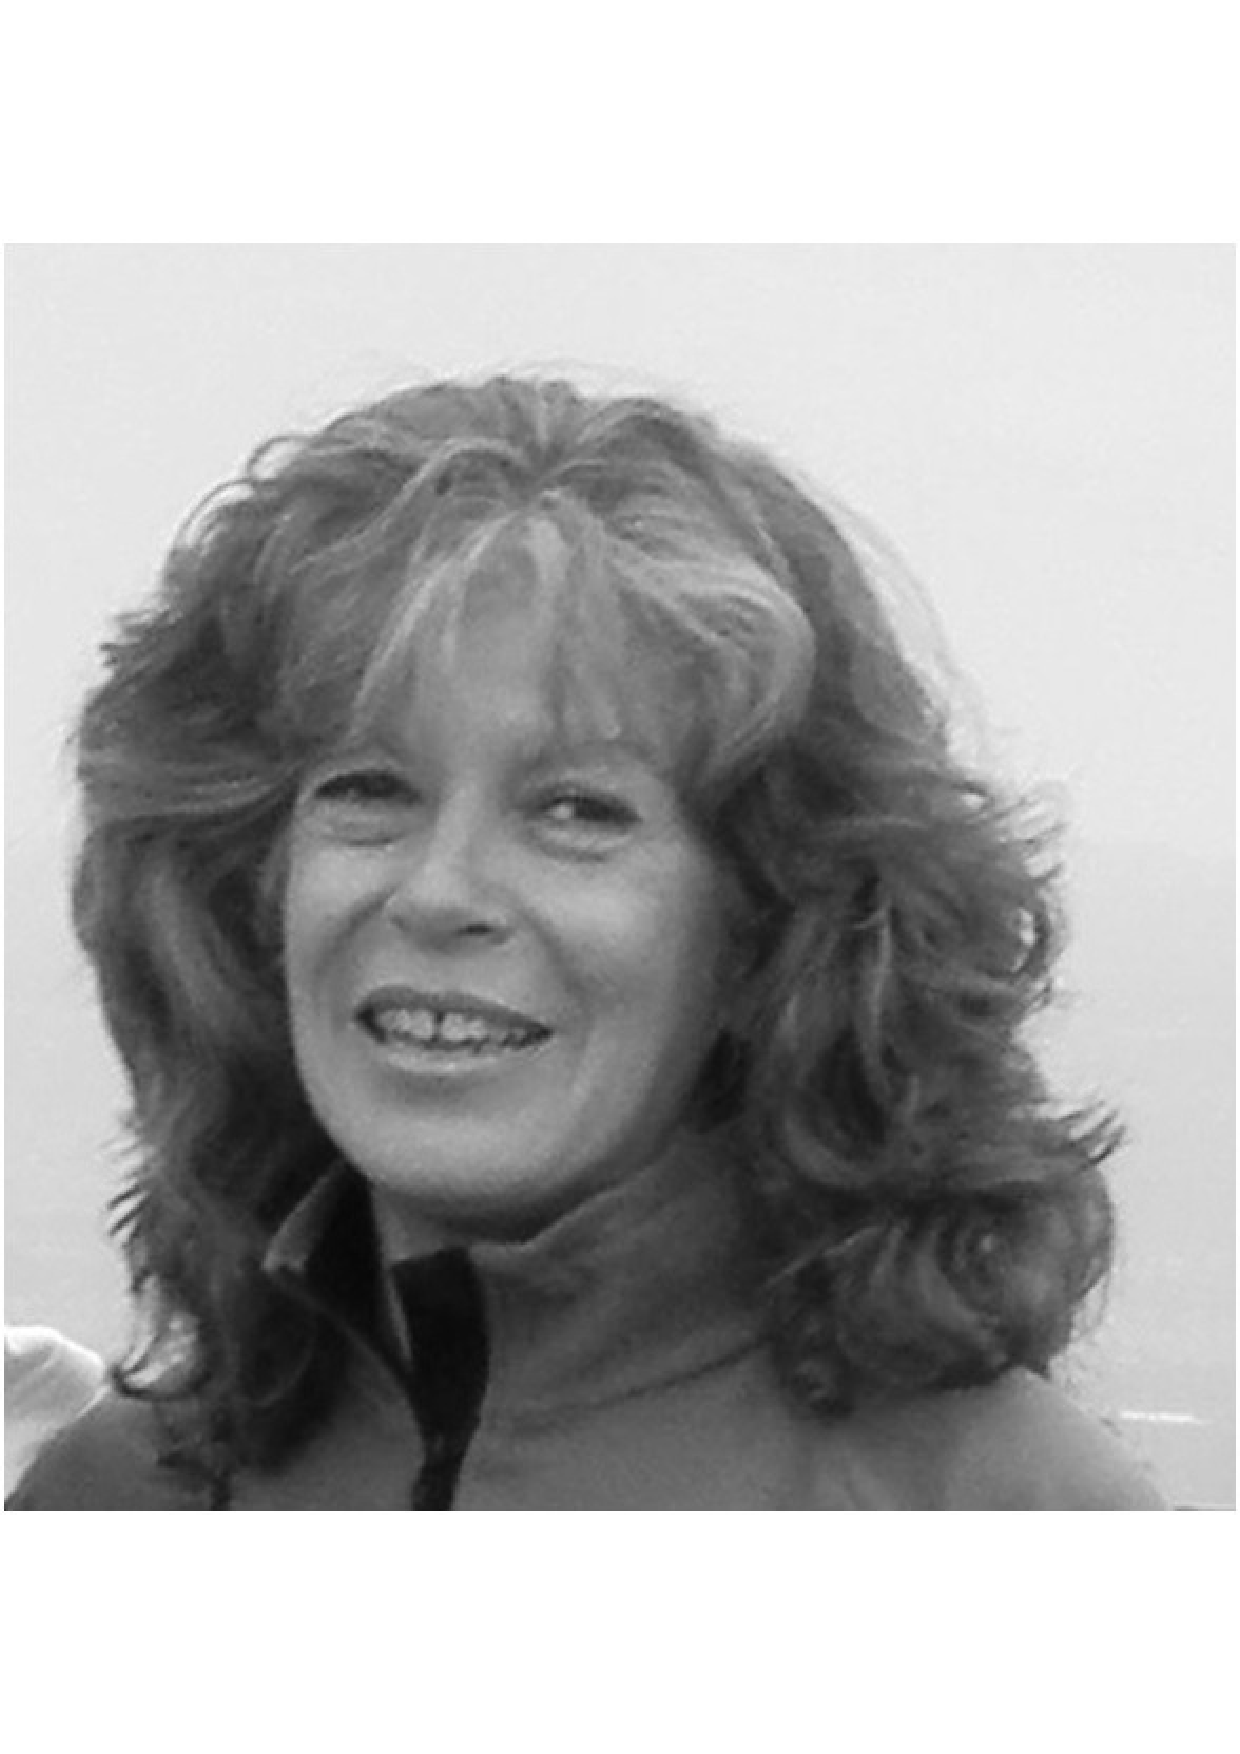
\includegraphics[height=1.8in,width=1.1in]{../../../Images/Fotos/JuliaGris7}}]{Julia Cassetti} 
%	received the B.Sc. degree in Mathematics and a postgraduate diploma in Mathematical Statistics, both from the Universidad de Buenos Aires (UBA), Argentina. \\
%	She is currently a Professor at the Universidad Nacional de General Sarmiento, Argentina.\\ 
%	Her research interests are in advanced statistical techniques in SAR image processing and applied statistics.
%\end{IEEEbiography}
%
%\begin{IEEEbiography}[{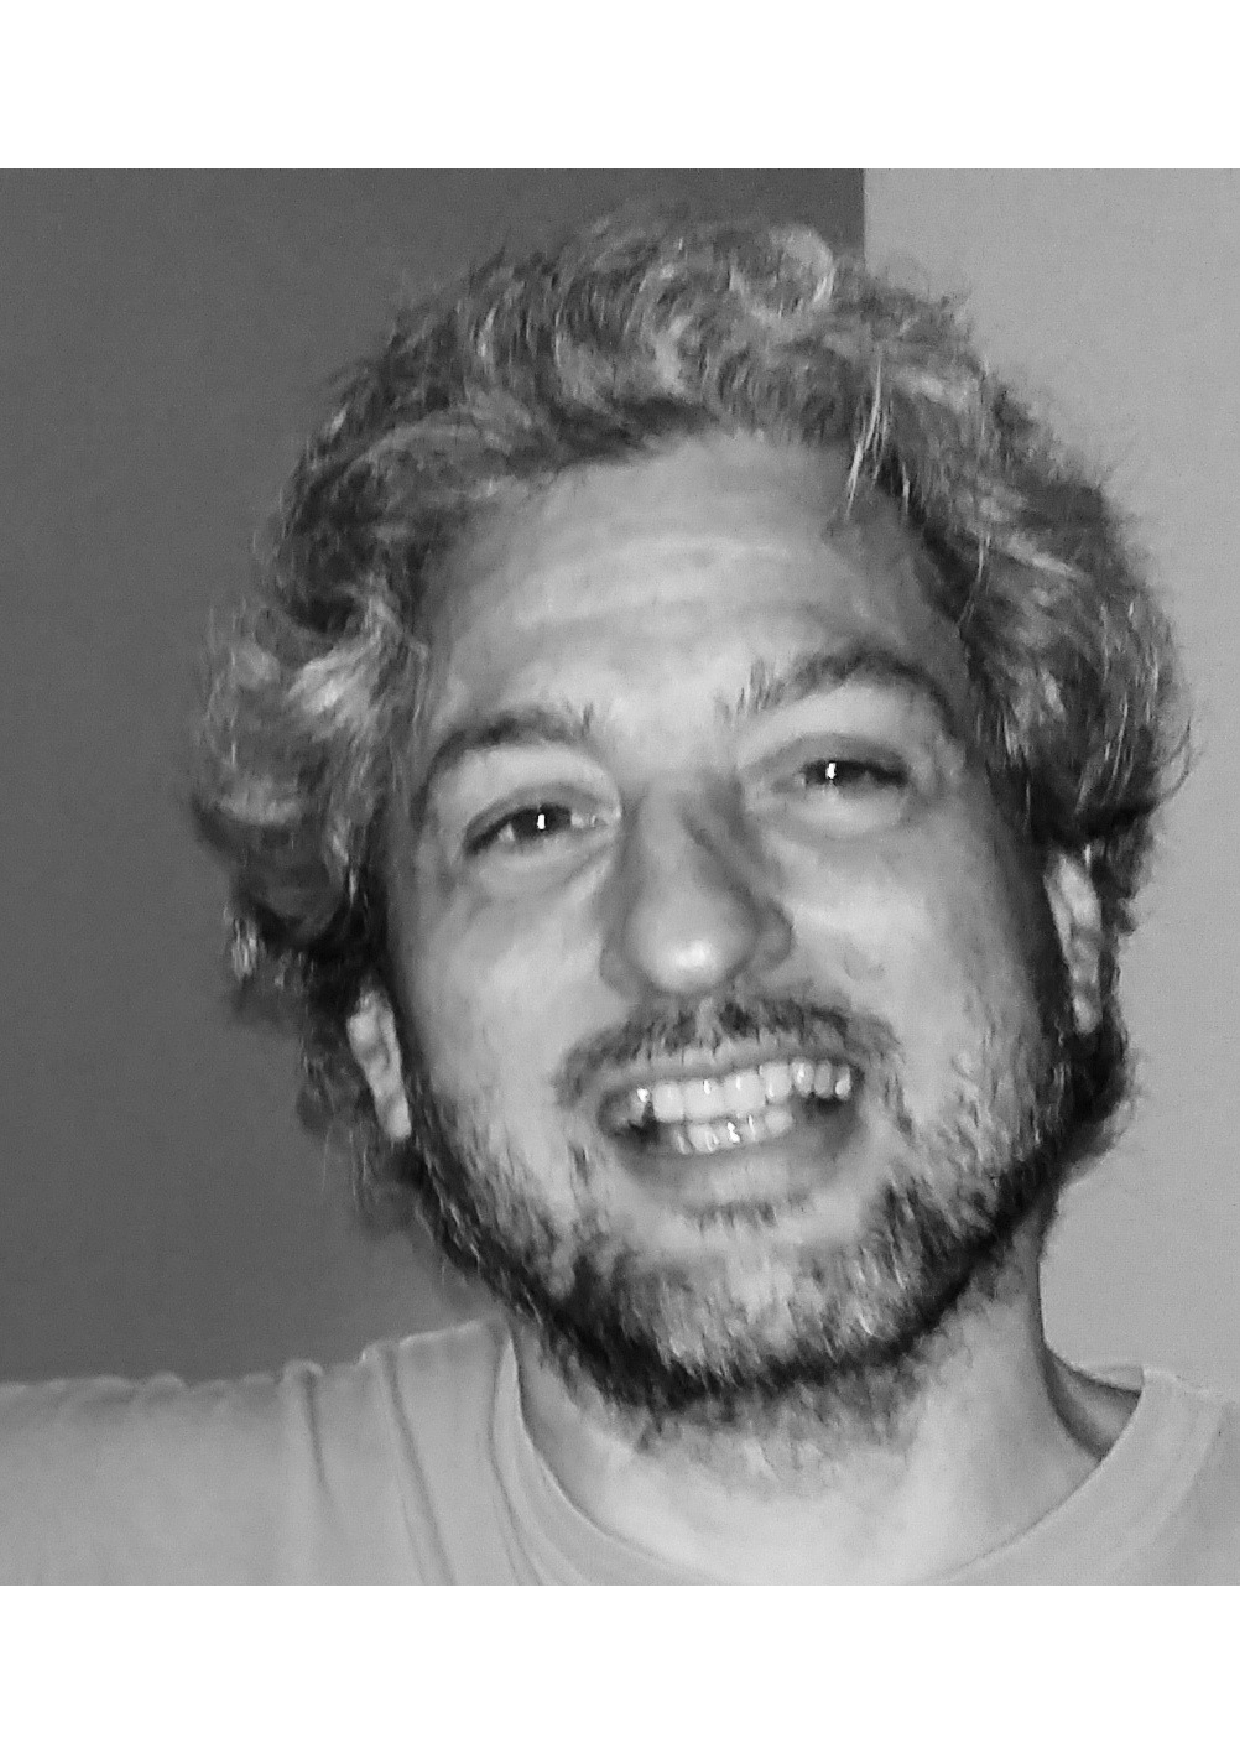
\includegraphics[scale=0.13]{../../../Im4218961ges/Fotos/Tico}}]{Diego Rial} 
%	received the B.Sc. degree in Mathematics from the Universidad de Buenos Aires, Argentina. His doctorate degree was in Science from the Instituto de Matem\'atica Pura e Aplicada (IMPA, Río de Janeiro).
%	He is currently an Associate Professor at Facultad de Ciencias Exactas y Naturales, Universidad de Buenos Aires. He is an Independent Researcher at CONICET - \textit{Consejo Nacional de Investigaciones Cient\'ificas y T\'ecnicas}, Argentina. His research interests are in nonlinear partial differential equations and numerical analysis.
%\end{IEEEbiography}
%
%\begin{IEEEbiography}[{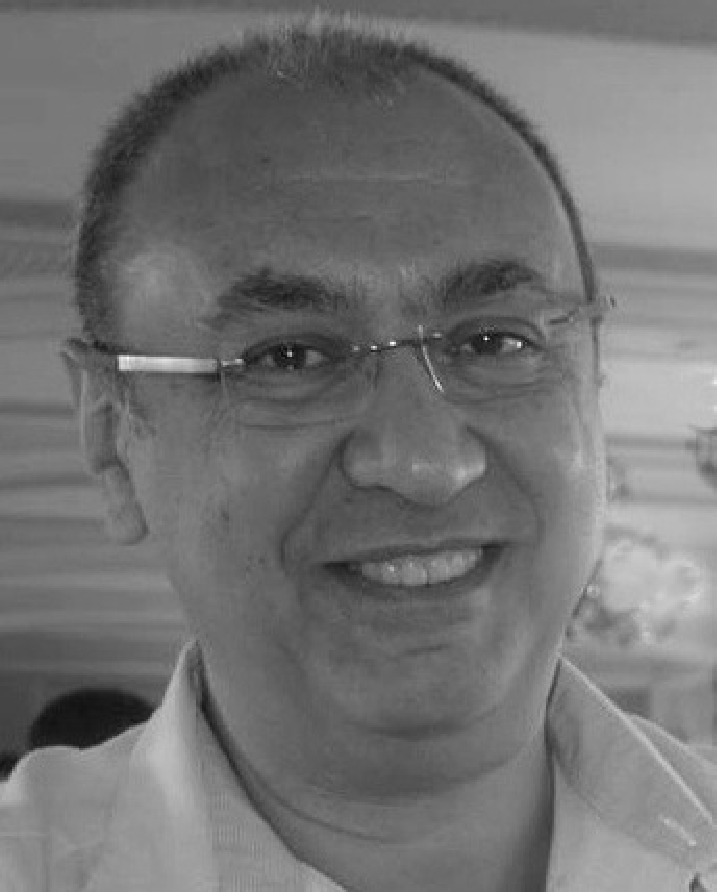
\includegraphics[width=1in]{../../../Images/Fotos/ACFrery_gray.pdf}}]{Alejandro C.\ Frery} (S'92--SM'03)
%	received the B.Sc. degree in Electronic and Electrical Engineering from the Universidad de Mendoza, Mendoza, Argentina.
%	His M.Sc. degree was in Applied Mathematics (Statistics) from the Instituto de Matem\'atica Pura e Aplicada (IMPA, Rio de Janeiro) and his Ph.D. degree was in Applied Computing from the Instituto Nacional de Pesquisas Espaciais (INPE, S\~ao Jos\'e dos Campos, Brazil).
%	He is currently the leader of LaCCAN -- \textit{Laborat\'orio de Computa\c c\~ao Cient\'ifica e An\'alise Num\'erica}, Universidade Federal de Alagoas, Macei\'o, Brazil.
%	His research interests are statistical computing and stochastic modelling.
%\end{IEEEbiography}

\end{document}